\documentclass[12pt,a4paper]{report}

\usepackage[utf8]{inputenc}
\usepackage{hyperref}
\usepackage{graphicx}
\title{Hesapsal Bilim}

\author{Öğretmen: Gilbert Strang \\ \\ Tercüme: Burak Bayramlı}

\date{}

\pagestyle{empty}
\begin{document}
\maketitle

\newpage

\begin{figure}[!hbp]
\center{
  \scalebox{0.45}{
  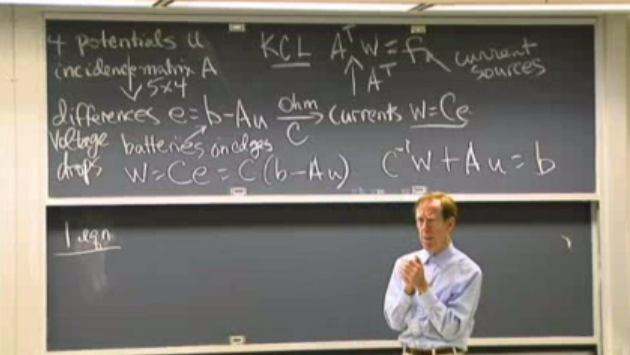
\includegraphics{strang.png}
  }
}
\end{figure}

\begin{center}

\vspace*{3cm}
Kaynak: OCW, MIT, Computational Science and Engineering, I, II\\
\vspace{0.5cm}
\url{https://ocw.mit.edu/courses/mathematics/18-085-computational-science-and-engineering-i-fall-2008} % end
\vspace{0.5cm}

Sayılar ve Kuramlar\\
\vspace{0.5cm}
\url{https://burakbayramli.github.io/dersblog/sk/}\\
\vspace{0.5cm}
Tüm Dosyalar, Kodlar\\
\vspace{0.5cm}
\url{https://github.com/burakbayramli/classnotes}\\
\end{center}


\end{document}

